\documentclass{beamer}

\mode<presentation>
 {\usetheme{CambridgeUS}
  \usecolortheme{beaver}
  \setbeamercovered{transparent}
  % appearance of bullets
  \useinnertheme{rectangles}
  \definecolor{mybullets}{rgb}{0.6,0.0,0.0}
  \setbeamercolor{structure}{fg=mybullets}

  \definecolor{mycolor}{rgb}{0.2,0.2,0.2}
  % bars
  %\setbeamercolor{section in toc}{fg=black,bg=white}
  %\setbeamercolor{alerted text}{fg=mycolor!80!gray}
  %\setbeamercolor*{palette primary}{fg=mycolor!60!black,bg=gray!30!white}
  %\setbeamercolor*{palette secondary}{fg=mycolor!70!black,bg=gray!15!white}
  %\setbeamercolor*{palette tertiary}{bg=mycolor!80!black,fg=gray!10!white}
  %\setbeamercolor*{palette quaternary}{fg=mycolor,bg=gray!5!white}
  %\setbeamercolor*{sidebar}{fg=mycolor,bg=gray!15!white}

  \setbeamercolor*{palette sidebar primary}{fg=mycolor!10!black}
  \setbeamercolor*{palette sidebar secondary}{fg=white}
  \setbeamercolor*{palette sidebar tertiary}{fg=mycolor!50!black}
  \setbeamercolor*{palette sidebar quaternary}{fg=gray!10!white}

  \setbeamercolor{titlelike}{parent=palette primary,fg=mycolor}
  \setbeamercolor{frametitle}{bg=gray!10!white}
  \setbeamercolor{frametitle right}{bg=gray!60!white}

  \setbeamercolor*{separation line}{}
  \setbeamercolor*{fine separation line}{}
}

 \def\Tiny{\fontsize{5pt}{5pt}\selectfont}
 \renewcommand{\arraystretch}{1.2}

% just show sections and subsections in table of contents
\setcounter{tocdepth}{2}


\usepackage[english]{babel}
\usepackage[latin1]{inputenc}

\usepackage{times}
\usepackage[T1]{fontenc}
\usepackage{eurosym}

\title[NES Project: Final Presentation]{Position Sensing and Imitation\\Final Presentation}

\author[Koslowski, Schmieder, Birk]{Konstantin Koslowski, Mathis Schmieder, Moksha Birk}

\institute[]
{TU Berlin \\
 Department of Telecommunication Systems \\
 Telecommunication Networks Group \\
}

\date{July 29th, 2015}

\pgfdeclareimage[height=0.5cm]{university-logo}{tu-tkn-logo.jpg}
\logo{\pgfuseimage{university-logo}}

\AtBeginSection{\frame{\begin{center}\huge\insertsection\end{center}}}

\begin{document}

\begin{frame}
  \titlepage
\end{frame}

\section{Introduction}
\subsection{Reminder}

\begin{frame}
  \frametitle{Reminder: Goal Statement}
  \begin{itemize}
    \item \textbf{Goal:} Mimic position and motion of a plate
    \vfill
    \item \textbf{Sensing:} 3D MEMS attitude sensor embedded in a plate
    \item \textbf{Communicating:} Implement industrial bus
    \item \textbf{Actuating:} Rotate a plate using motors
  \end{itemize}
\end{frame}

%\section{Overview}
%\subsection{Sensing}
%\begin{frame}
  %\frametitle{Milestone: Sensing}
  %\framesubtitle{Read and process MEMS data}
  %\textbf{Status:}
  %\begin{itemize}
    %\item Reading data via I2C works
    %\item Computing plate position from data works
    %\item Additional filtering might be required
  %\end{itemize}
%\end{frame}
%
%\subsection{Actuation}
%\begin{frame}
  %\frametitle{Milestone: Actuation}
  %\framesubtitle{Control stepper motors}
  %\textbf{Status:}
  %\begin{itemize}
    %\item Communication with stepper drivers via SPI works
    %\item Control of stepper motors works
    %\item Additional work on control daemon necessary
  %\end{itemize}
%\end{frame}
%
%\subsection{Mechanics}
%\begin{frame}
  %\frametitle{Milestone: Mechanics}
  %\framesubtitle{Construct movable plate}
  %\textbf{Status:}
  %\begin{itemize}
    %\item First version of plate construction printed
    %\item Works for now
    %\item Design on second, refined version in progress
  %\end{itemize}
%\end{frame}
%
%\subsection{Communication}
%\begin{frame}
  %\frametitle{Milestone: Communication}
  %\framesubtitle{Implement industrial bus}
  %\textbf{Status:}
  %\begin{itemize}
    %\item A lot of research was done
    %\item EtherCAT selected as most interesting
    %\item We couldn't get EtherCAT working
    %\item CAN used as fallback
  %\end{itemize}
%\end{frame}
%
%\subsection{Controller}
%\begin{frame}
  %\frametitle{Milestone: Controller}
  %\framesubtitle{Bus master, main computational unit}
  %\textbf{Status:}
  %\begin{itemize}
    %\item Modular design to fit CAN and EtherCAT
    %\item High-level controller class
      %\begin{itemize}
        %\item Receives periodic sensor input events
        %\item Computes angle corrections for all drives
      %\end{itemize}
    %\item CAN wrapped into classes to provide the events and send corrections
    %\item Component interaction via Sockets
    %\item Built on a BeagleBone Black
  %\end{itemize}
%\end{frame}


\section{System Specifications}
\subsection{Functional Overview}
\begin{frame}
  \frametitle{Functional Overview}
\begin{figure}
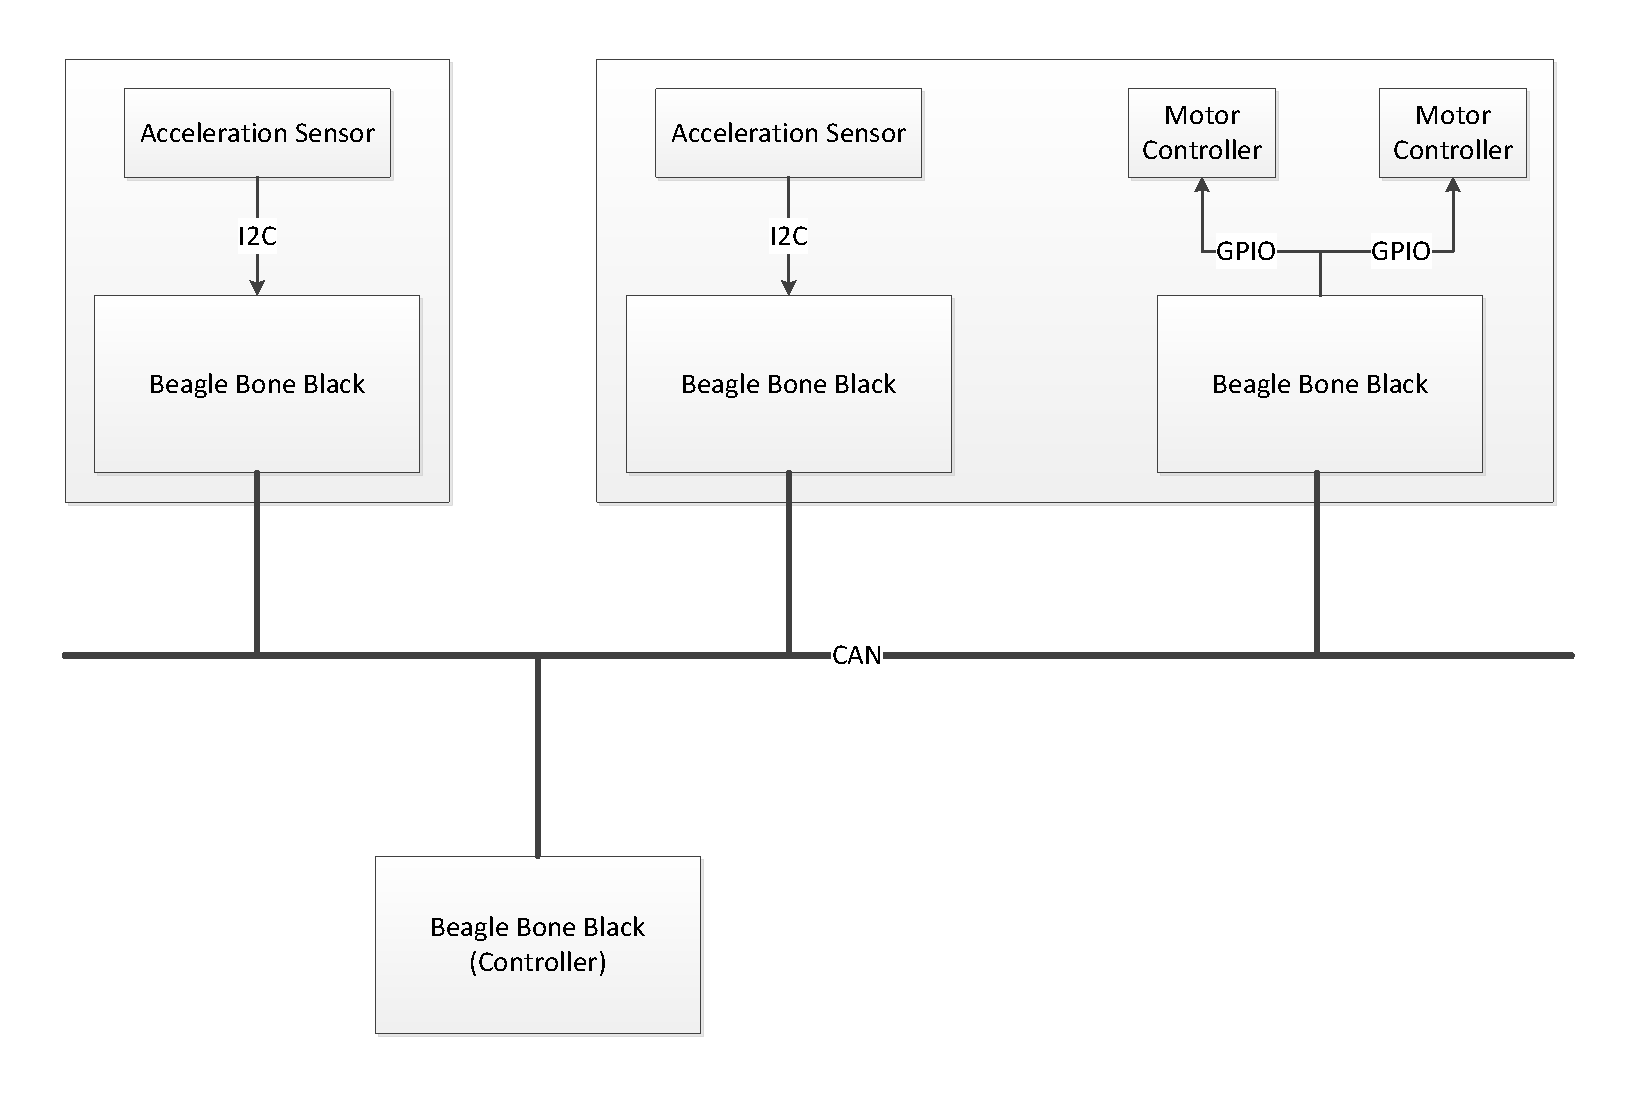
\includegraphics[width=0.7\textwidth]{functional_specification_can.pdf}
\caption{Diagram of the Functional Specification}
\end{figure}
\end{frame}

%\subsection{Timing}
%\begin{frame}
  %\frametitle{Timing}
  %\textbf{Timing goal:} Move plate to desired position within 1 second
%
  %\vfill
%
  %\textbf{Fixed timings:}
  %\begin{itemize}
    %\item Sensors
      %\begin{itemize}
        %\item Sample every 10 ms
        %\item Report mean value every 100 ms
      %\end{itemize}
    %\item Actuation takes up to 500 ms
  %\end{itemize}
%
  %\vfill
%
  %\textbf{Delay constraint:} 500 ms to compute \& communicate
%\end{frame}

\subsection{Bus Design}
\begin{frame}
  \frametitle{Bus}
  \framesubtitle{Bus specification}
  \begin{itemize}
    \item EtherCAT could not be implemented due to
		\begin{itemize}
			\item Unsuccessful installation of SDK on Linux
			\item Problems with Ethernet NIC incompatibilities 
		\end{itemize}
		\vfill
    \item Using fallback option CAN
		\begin{itemize}
			\item All nodes are BeagleBone Blacks
			\item CAN controller: SN65HVD230
			%\item Sensor values are periodically fed to the Controller from a buffer
		\end{itemize}
  \end{itemize}
\end{frame}

\subsection{CAN Design}
\begin{frame}
  \frametitle{CAN}
  \framesubtitle{Bus Design}
	Reminder:
	\begin{itemize}
		\item \textbf{Timing goal:} Move plate to desired position within 1 second
		\item Actuation takes up to 500\,ms
		\item Sensors report mean value every 100\,ms
	\end{itemize}
	\vfill
  \begin{itemize}
    \item Required cycle time: 100\,ms
    \item Sensor values are periodically fed to the Controller from a buffer
    \item Controller computes movement commandos and sends them to the drivers
  \end{itemize}
\end{frame}

\subsection{Message IDs}
\begin{frame}
  \frametitle{Messsage ID Descriptions}
  \begin{table}
\begin{tabular}{l | c | c }
Node Name & ID / Priority & Master / Slave \\
\hline \hline
Controller & 1 & Master \\
Source Sensor & 2 & Slave \\
Target Sensor & 3 & Slave \\
Stepper Driver & 4 & Slave
\end{tabular}
\caption{Nodes in the network}
\end{table}
\end{frame}

\subsection{Messages}
\begin{frame}
  \frametitle{Message Description}
  \framesubtitle{Bus Option 2}
  \begin{table}
\begin{tabular}{l | c | c }
Description & Data Request & Length \\
\hline \hline
Sensor Position   & Allowed     & 6 Bytes \\
Motor Status      & Allowed     & 4 Bytes \\
Rotation Command  & Not Allowed & 3 Bytes \\
Reset Command     & Not Allowed & 3 Bytes
\end{tabular}
\caption{Possible messages in the network}
\end{table}
\end{frame}

\begin{frame}
  \frametitle{Message Sequence Charts}
  \framesubtitle{}
  \begin{itemize}
    \item ?
  \end{itemize}
\end{frame}

\begin{frame}
  \frametitle{}
  \framesubtitle{}
  \begin{itemize}
    \item ?
  \end{itemize}
\end{frame}

\section{Discussion}
\begin{frame}
  \frametitle{Thanks for your attention!}
  \huge{Questions? Ideas? Suggestions?}
\end{frame}

\end{document}
